\chapter{Pure Data Patches}\label{ap:pd_patches}
\Todo{make the patches more readable and replace the pics}

\section{Filter Based Additive Synthesis}
\begin{figure}[H]
  \centering
    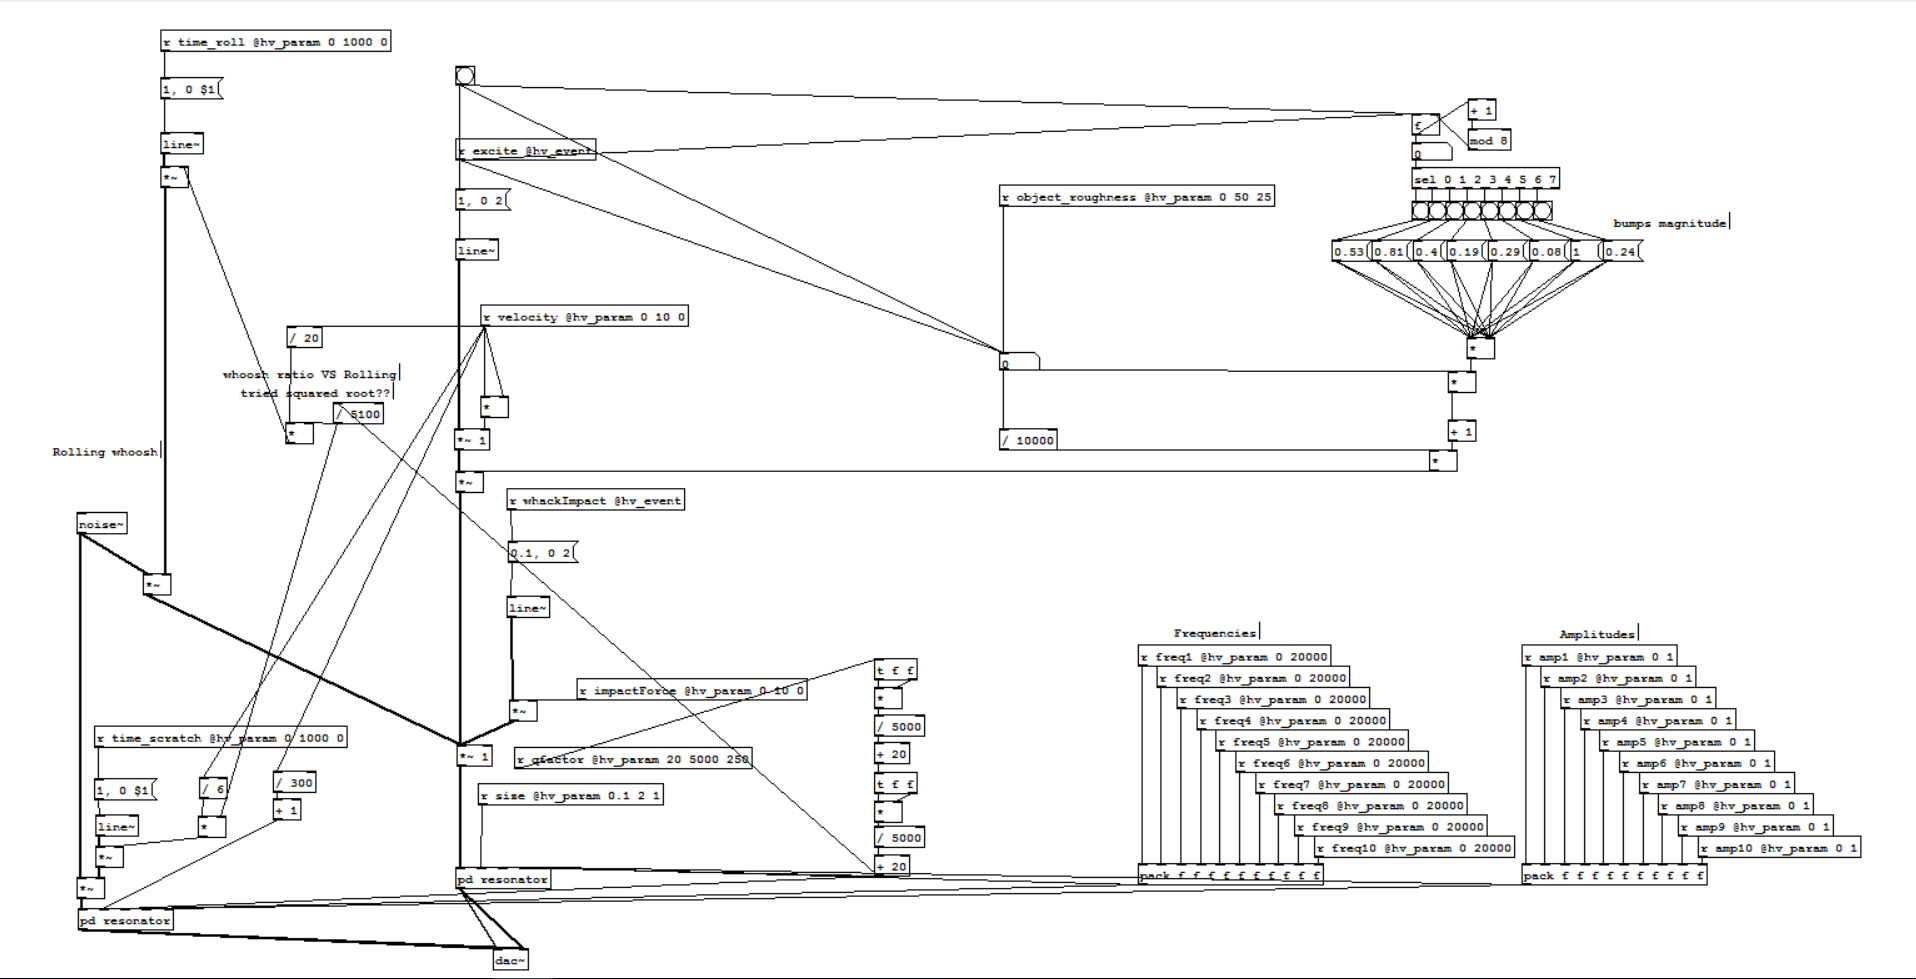
\includegraphics[width=\textwidth]{PdPatches/FBmain.PNG}
      \caption{The main Pure Data patch for the filter-based additive synthesis.}
      \label{fig:FBmain}
\end{figure}

\begin{figure}[H]
  \centering
    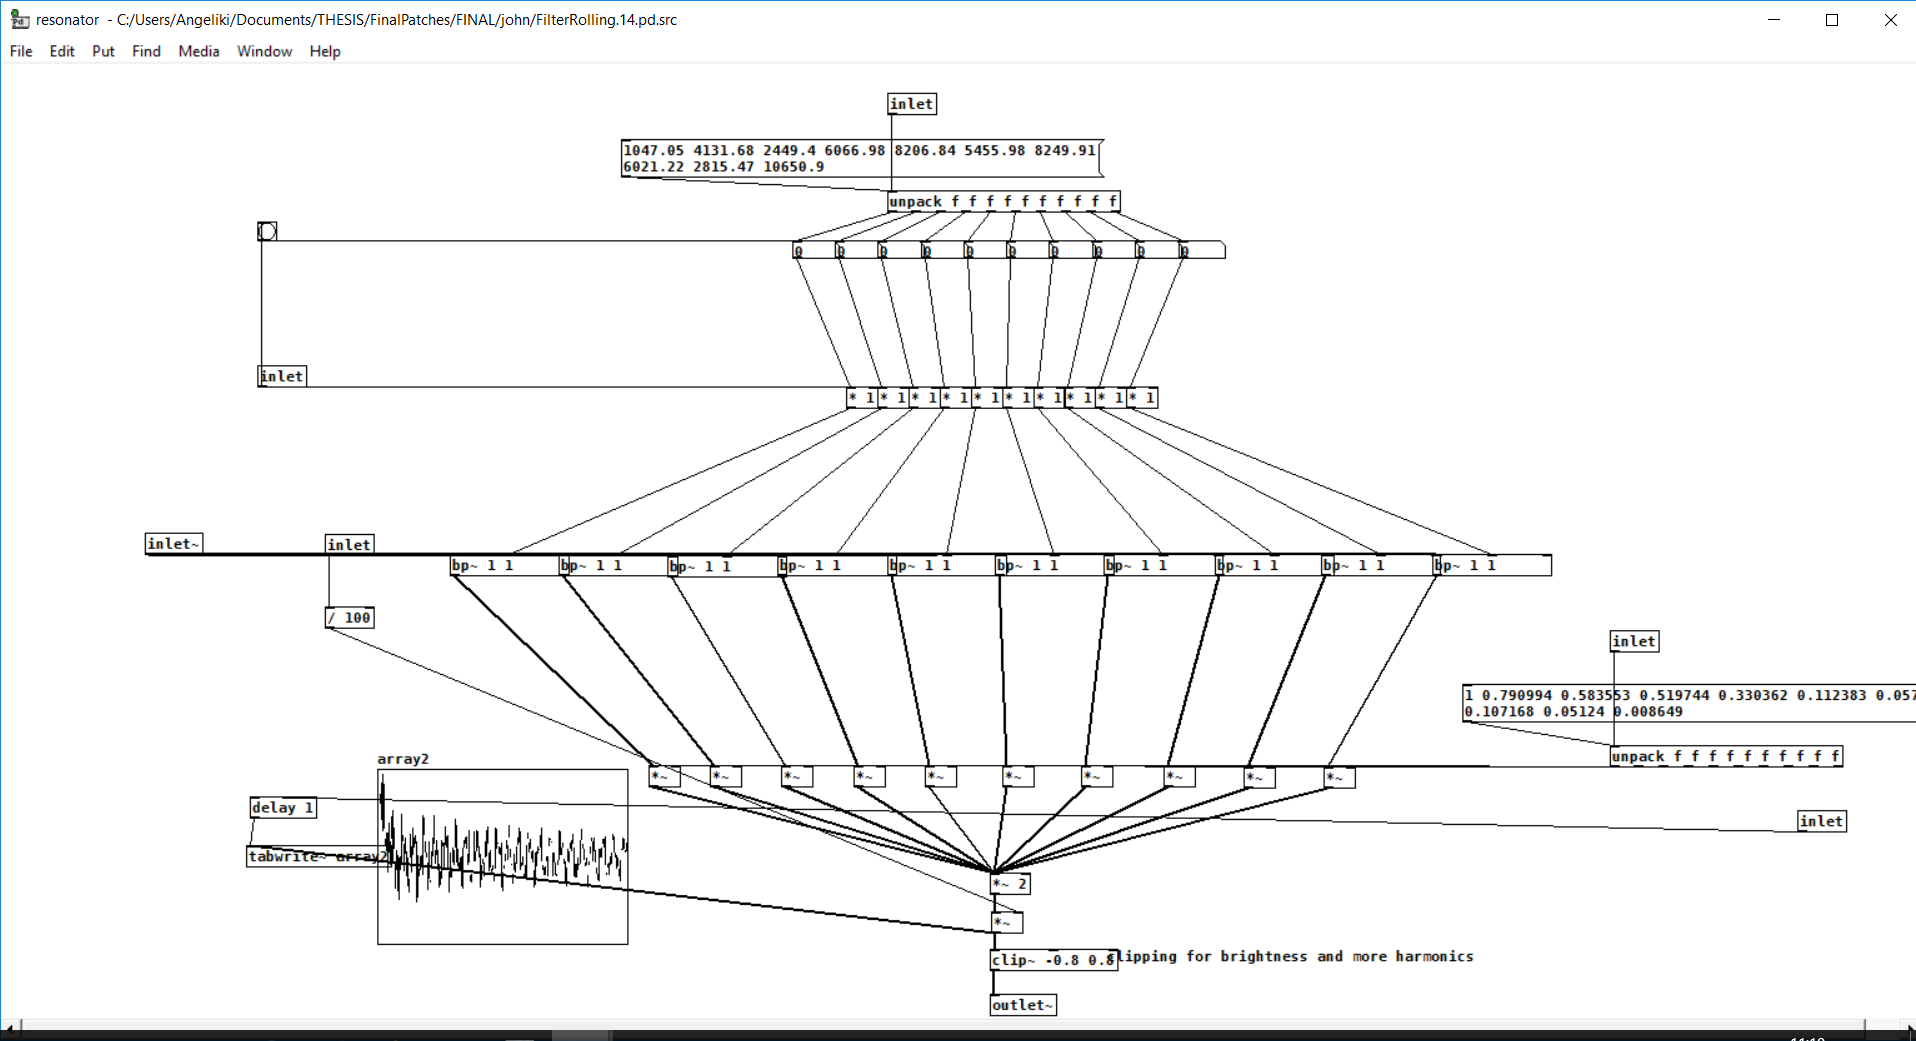
\includegraphics[width=\textwidth]{PdPatches/FBresonator.PNG}
      \caption{The resonator Pure Data patch for the filter-based additive synthesis.}
      \label{fig:FBres}
\end{figure}

\section{Sinusoidal Additive Synthesis}

\begin{figure}[H]
  \centering
    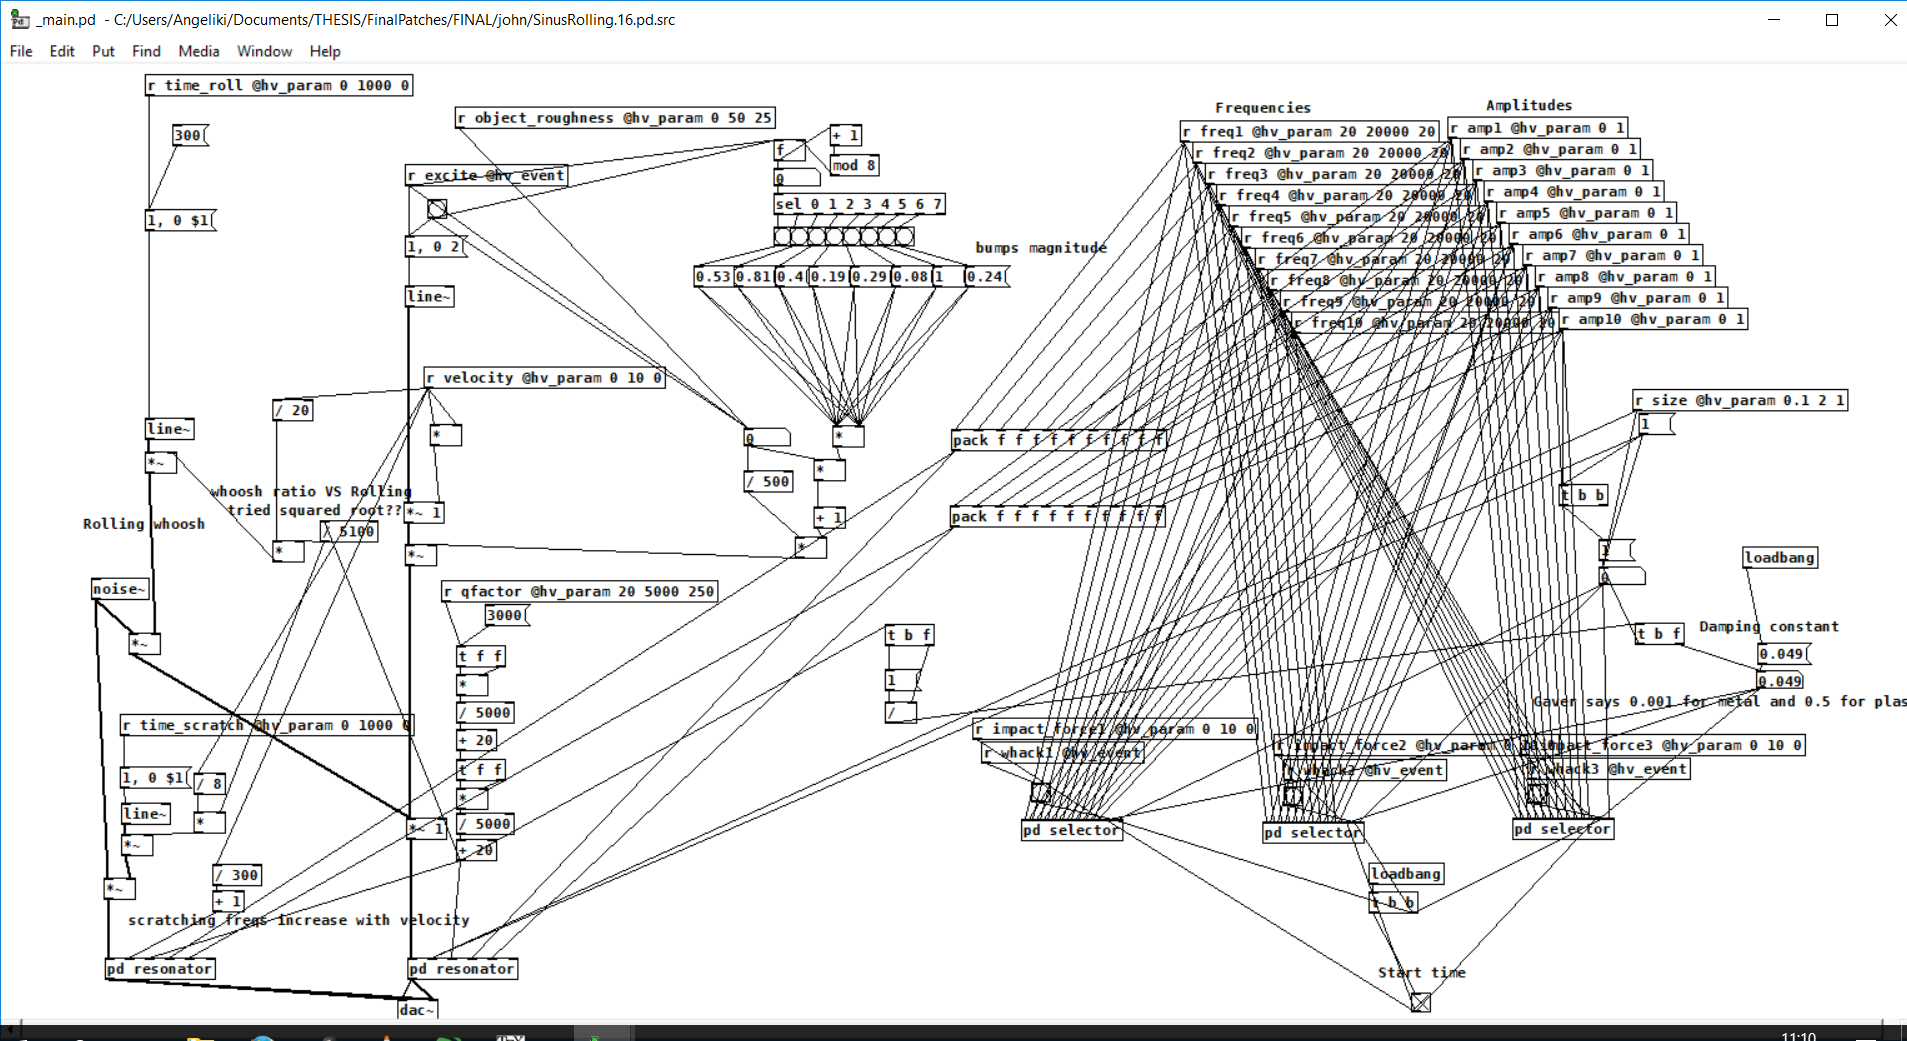
\includegraphics[width=\textwidth]{PdPatches/Smain.PNG}
      \caption{The main Pure Data patch for the sinusoidal additive synthesis.}
      \label{fig:Smain}
\end{figure}

\begin{figure}[H]
  \centering
    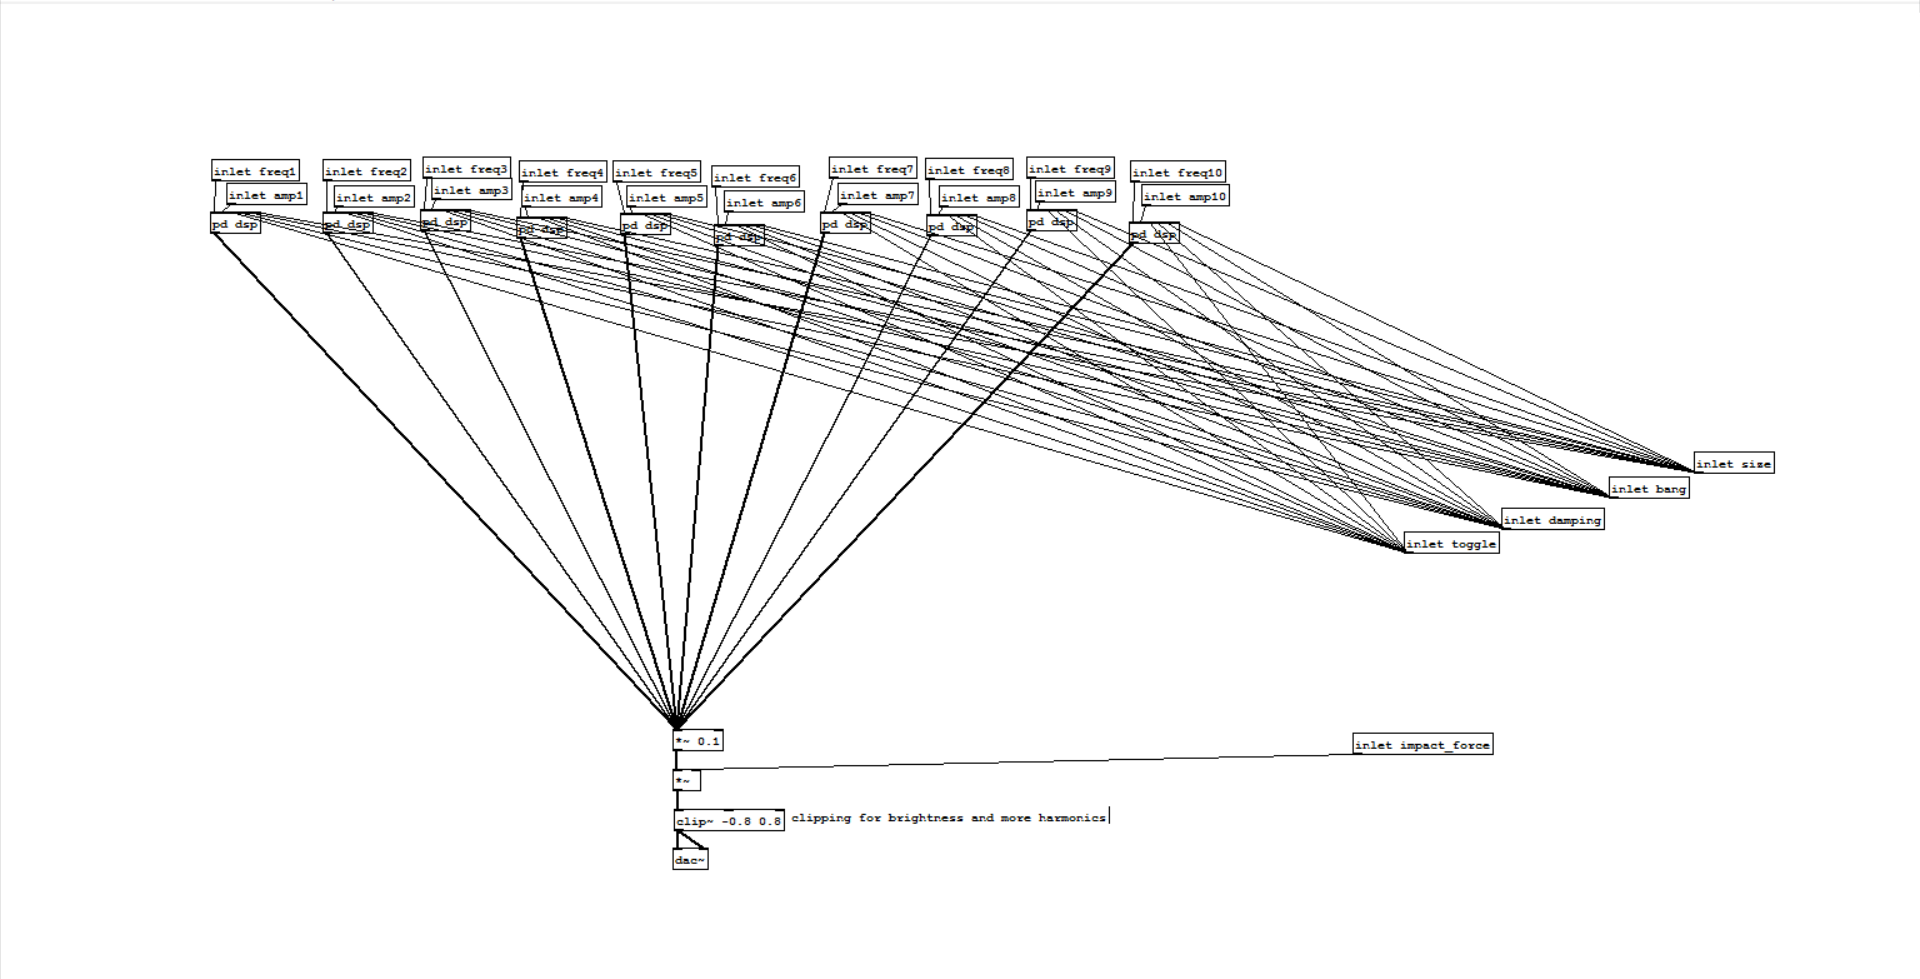
\includegraphics[width=\textwidth]{PdPatches/Sselector.PNG}
      \caption{The selector Pure Data patch for the filter-based additive synthesis.}
      \label{fig:Ssel}
\end{figure}

\begin{figure}[H]
  \centering
    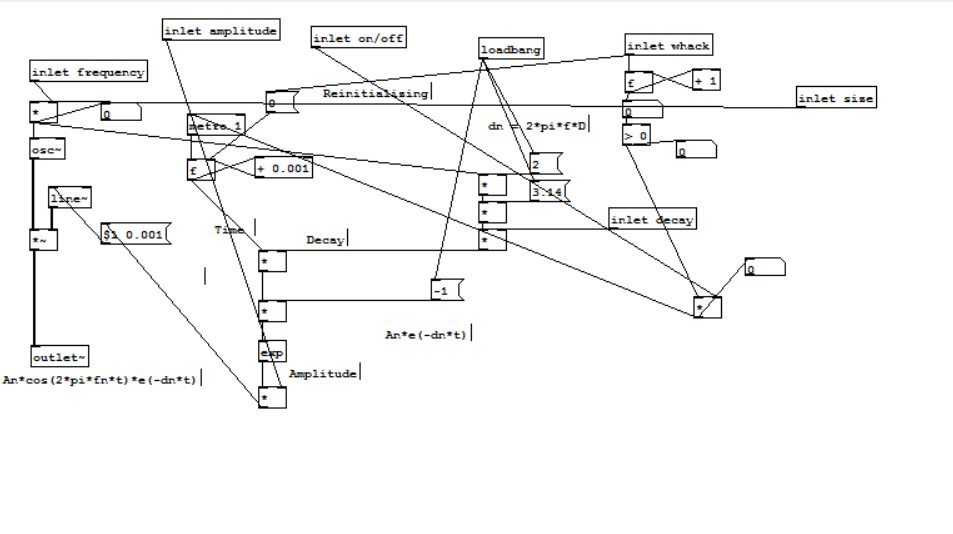
\includegraphics[width=\textwidth]{PdPatches/Sdsp.PNG}
      \caption{The dsp Pure Data patch for the filter-based additive synthesis.}
      \label{fig:Sdsp}
\end{figure}

\chapter{Instructions for the Subjective Experiments}
\Todo{should we include it or not?}

\chapter{Spectrograms}\label{ap:spectrograms}
Spectrograms of one object from each material used in this study. Each graph represents sound coming from one ``sound area'' of the object, either from the real-world recording or from the two synthesis methods (Sinusoidal Additive Synthesis and Filter-based Modal Synthesis).
\section*{Plastic bowl}

\begin{figure}[H]
  \centering
    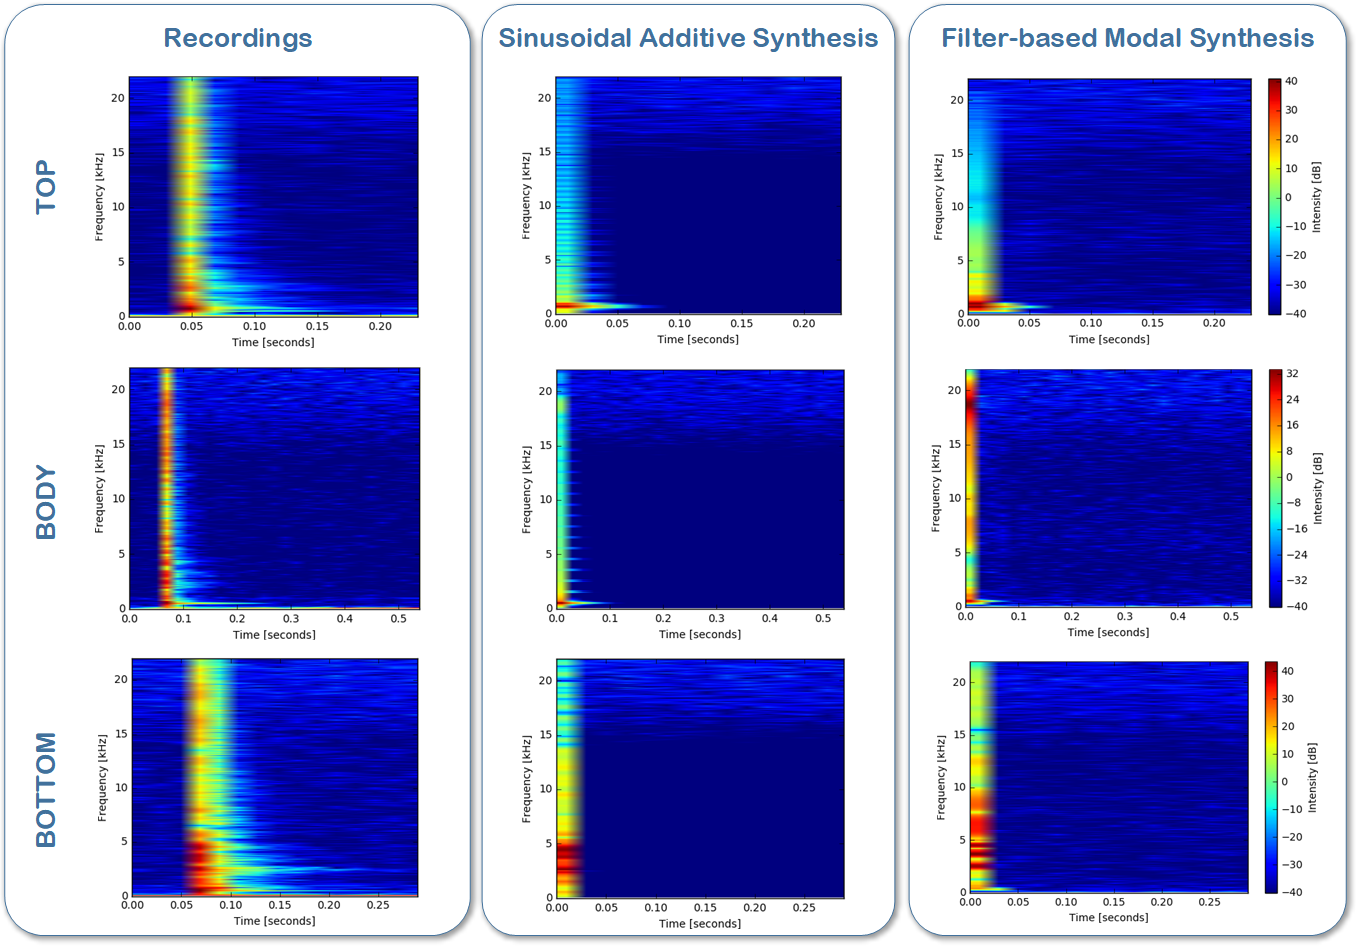
\includegraphics[width=\textwidth]{specs/bowl.png}
      \caption{Spectrograms of recordings and the two synthesis methods for the plastic bowl.}
      \label{fig:sp_bowl}
\end{figure}

\newpage

\section*{Wooden mortar}

\begin{figure}[H]
  \centering
    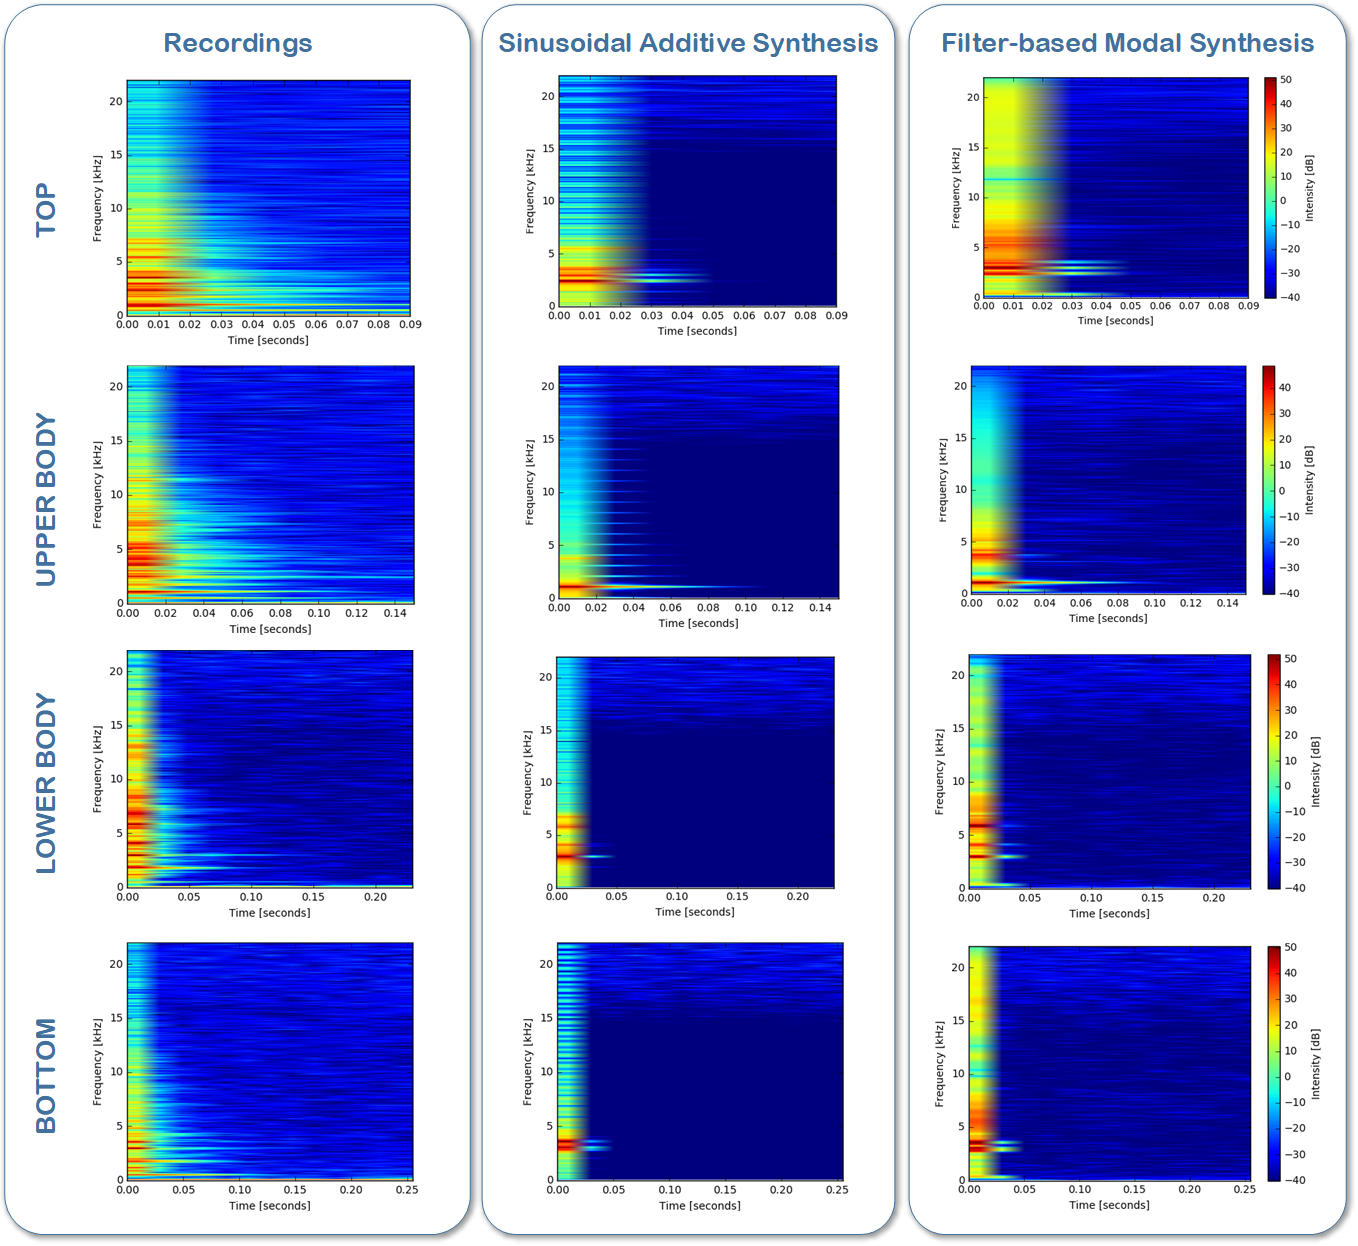
\includegraphics[width=\textwidth]{specs/mortar.png}
      \caption{Spectrograms of recordings and the two synthesis methods for the wooden mortar.}
      \label{fig:sp_mortar}
\end{figure}

\newpage

\section*{Ceramic plate}

\begin{figure}[H]
  \centering
    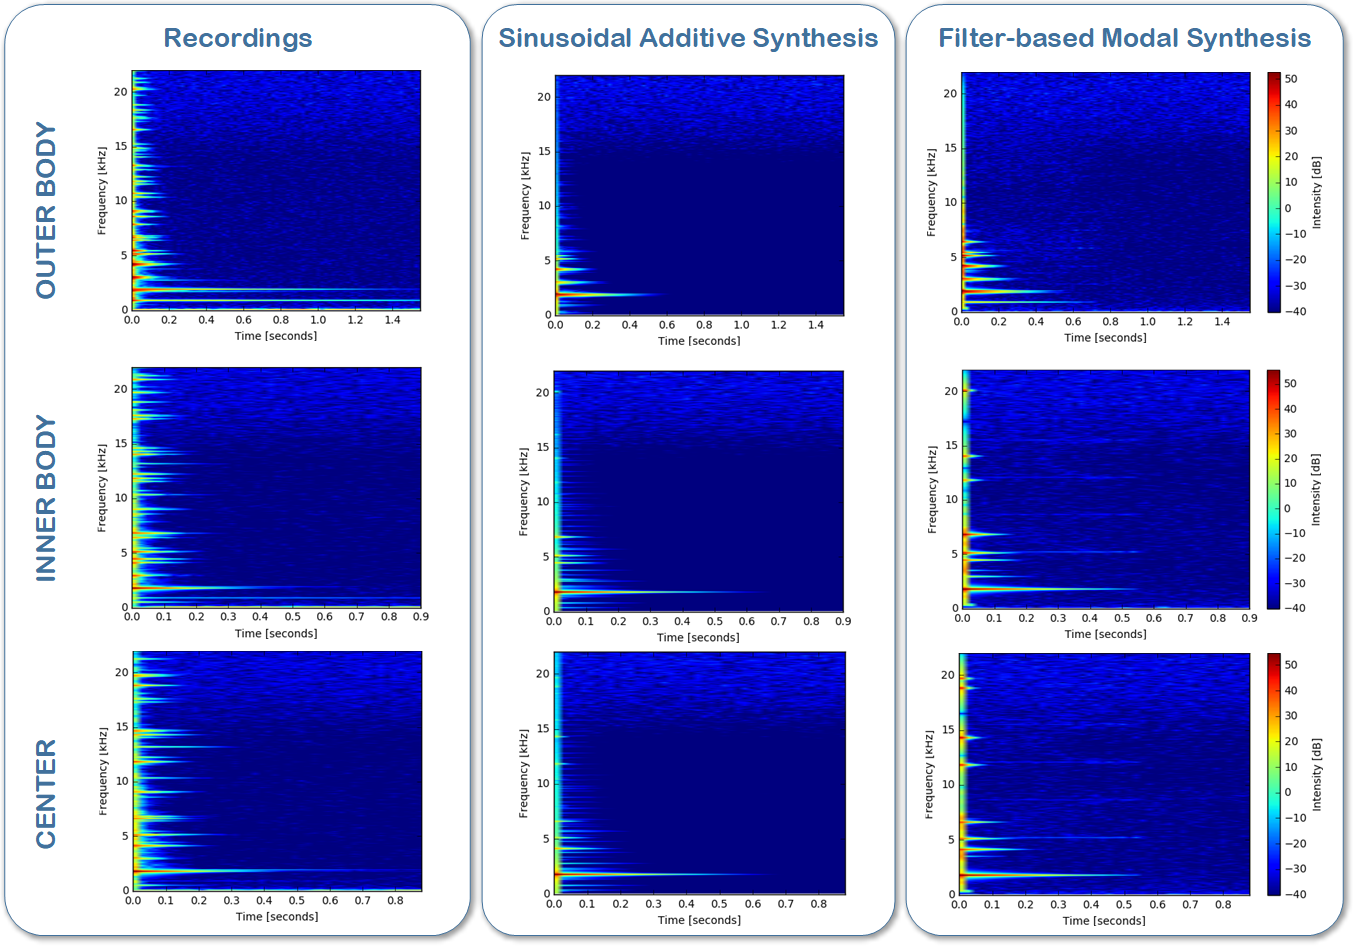
\includegraphics[width=\textwidth]{specs/plate.png}
      \caption{Spectrograms of recordings and the two synthesis methods for the ceramic plate.}
      \label{fig:sp_plate}
\end{figure}

\newpage

\section*{Wine glass}

\begin{figure}[H]
  \centering
    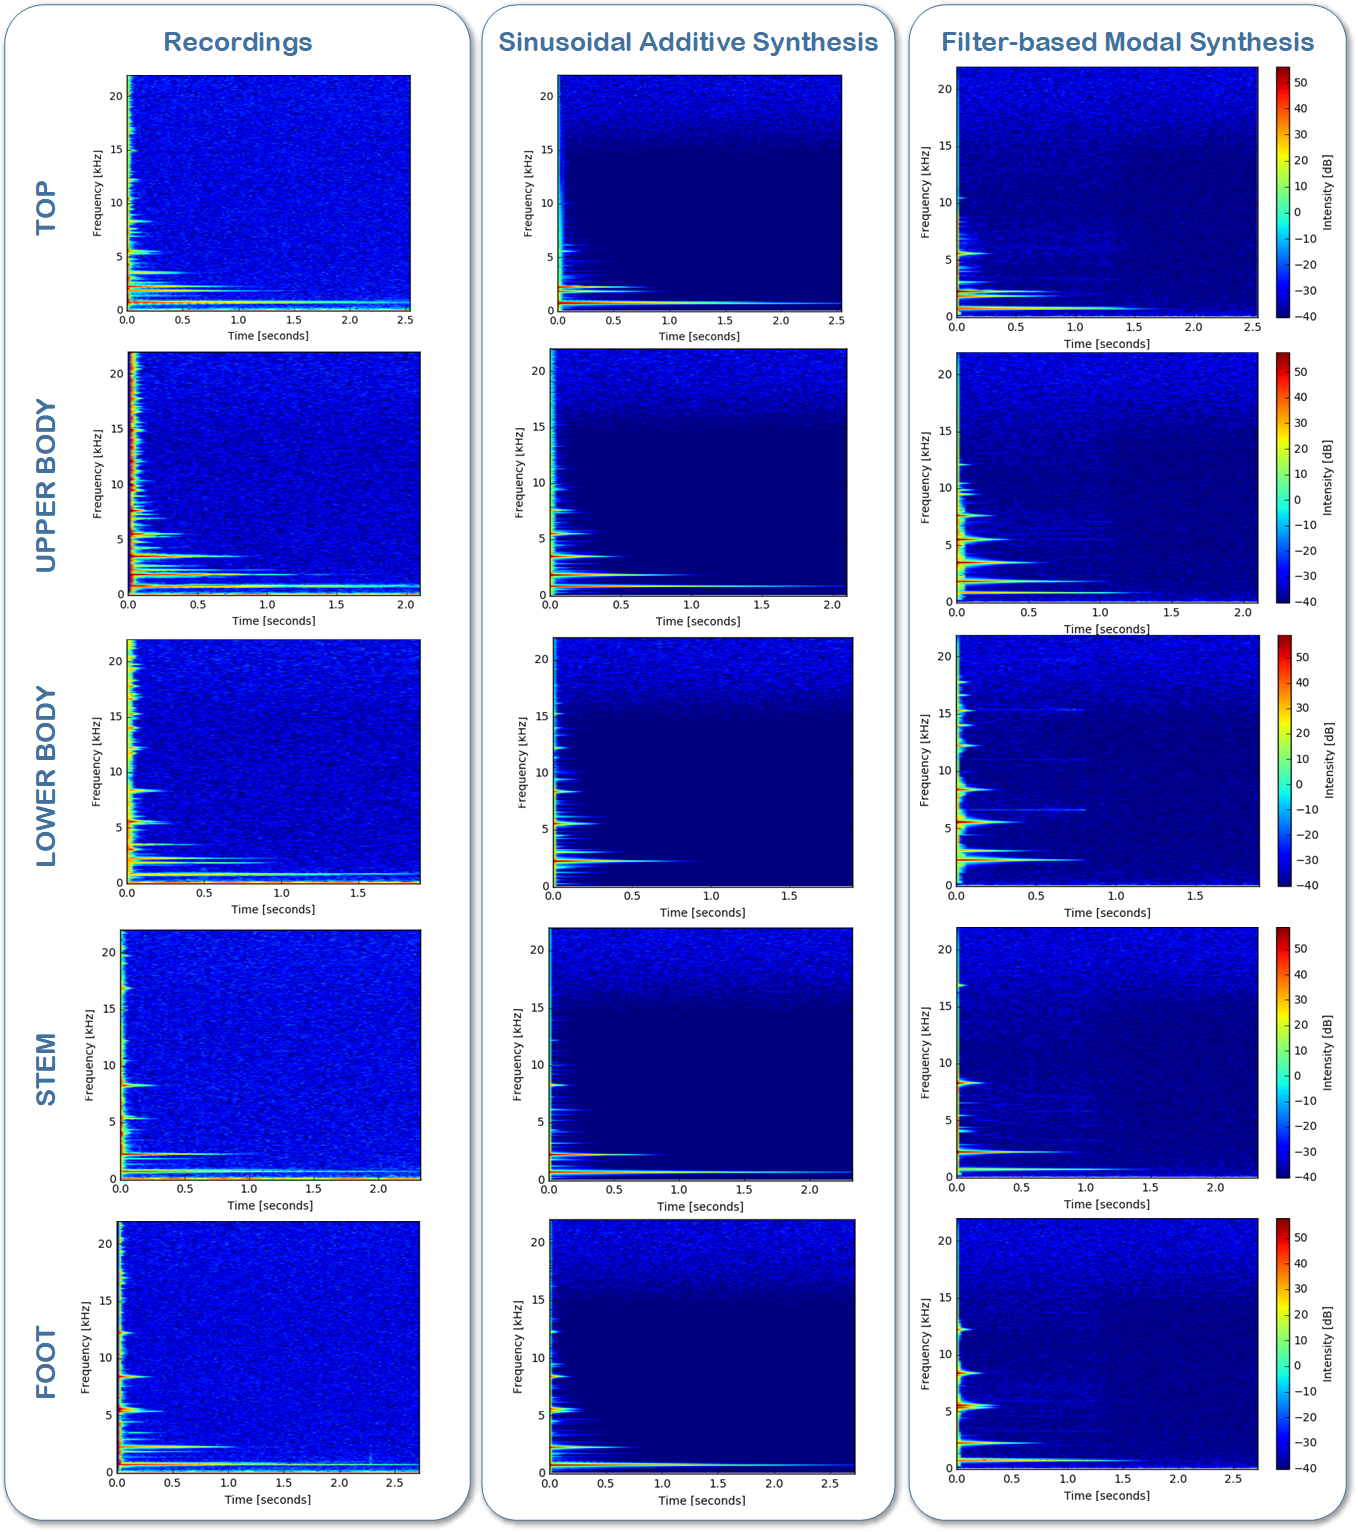
\includegraphics[width=\textwidth]{specs/glass.png}
      \caption{Spectrograms of recordings and the two synthesis methods for the wine glass.}
      \label{fig:sp_glass}
\end{figure}

\newpage

\section*{Metallic wok}

\begin{figure}[H]
  \centering
    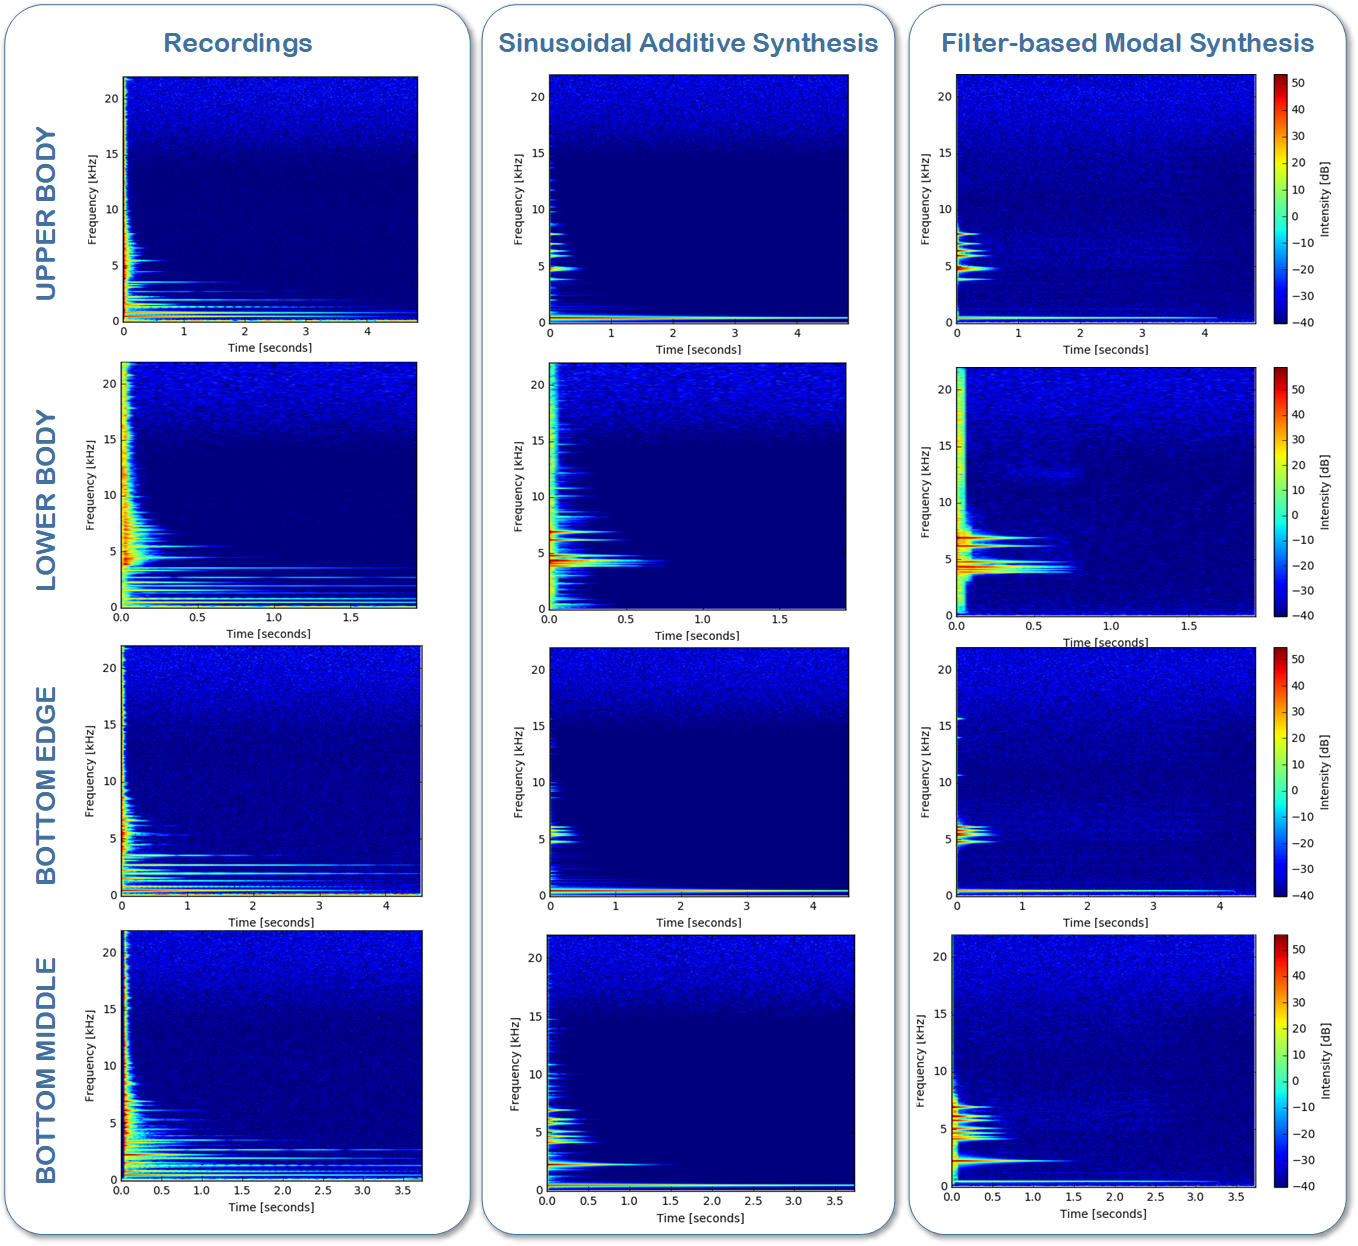
\includegraphics[width=\textwidth]{specs/wok.png}
      \caption{Spectrograms of recordings and the two synthesis methods for the metallic wok.}
      \label{fig:sp_wok}
\end{figure}

\newpage

\chapter{User Guide to our Product}\label{ap:guide}

\begin{itemize}
\item Decide on the areas to separate the object
\item Record impact sounds
\item Put audio files into the data extraction algorithm
\item Measure object perimeter and weight of the object
\item Put all data in Unity\textsuperscript{\textregistered} in Data Script
\item Make a new item entry in Unity\textsuperscript{\textregistered}'s Audio Manager Script
\item Make an FBX\textsuperscript{\textregistered} model of your object with the same dimensions and put it into a Unity\textsuperscript{\textregistered} scene as game object
\item Assign the Audio Manager to the game object
\item Tag the game object with the corresponding tag
\item Adjust the material, size and object roughness sliders
\end{itemize}


